\section{Tổng Quan và Mục Tiêu Bài Thực Hành 2}

\subsection{Giới thiệu}
Bài thực hành 2 tập trung vào các cơ chế đồng bộ và giao tiếp giữa các tiến trình (Inter-Process Communication - IPC) trong hệ điều hành thời gian thực Zephyr RTOS trên Kit thí nghiệm BKIT ARM4 (STM32F407ZGT6). Nội dung khảo sát việc ứng dụng Binary Semaphore, Counting Semaphore, Mutex và Message Queue nhằm giải quyết triệt để các bài toán kinh điển trong lập trình hệ thống nhúng: điều phối thứ tự thực thi tuần tự, loại trừ lẫn nhau bảo vệ vùng găng, và truyền nhận dữ liệu an toàn phi phong tỏa giữa ngắt phần cứng (ISR) với luồng thực thi (Thread).

\subsection{Mục tiêu bài thực hành}
\begin{itemize}
    \item Vận dụng Binary Semaphore để thiết lập trật tự thực thi nghiêm ngặt giữa nhiều thread chạy song song.
    \item Sử dụng Semaphore có cơ chế Timeout để phát hiện mất tín hiệu định kỳ và xử lý an toàn lỗi ngắt.
    \item Kết hợp Counting Semaphore và Mutex để quản lý hồ tài nguyên dùng chung (Resource Pool) gồm 2 kênh phần cứng cho 4 tác vụ đồng thời.
    \item Thực hiện giao tiếp một chiều bất đồng bộ giữa ISR và Thread thông qua Message Queue, phân tích hiện tượng tràn bộ đệm khi mất cân bằng thông lượng.
    \item Thiết kế hệ thống đèn giao thông thông minh hoàn chỉnh: máy trạng thái FSM, ngắt nút bấm người đi bộ, và kiến trúc ghi log tập trung qua Message Queue.
\end{itemize}

\subsection{Quy định kỹ thuật bắt buộc}
\begin{itemize}
    \item Tuyệt đối không chờ bằng vòng lặp rỗng hỏi vòng (\texttt{while (!flag) \{\}}) hay \texttt{k\_busy\_wait()}: mọi sự đồng bộ phải dùng Semaphore, Mutex hoặc Message Queue.
    \item Trong ngữ cảnh ngắt ISR: Chỉ sử dụng các API non-blocking với tham số \texttt{K\_NO\_WAIT}; tuyệt đối không gọi \texttt{k\_msleep}, \texttt{k\_mutex\_lock}, hay \texttt{printf}.
    \item Khởi tạo tĩnh các đối tượng kernel bằng các macro chuẩn: \\
    \texttt{K\_SEM\_DEFINE}, \texttt{K\_MUTEX\_DEFINE}, và \texttt{K\_MSGQ\_DEFINE}.
    \item Mọi thread phải được khởi tạo bằng \texttt{K\_THREAD\_DEFINE} với đúng định danh và độ ưu tiên theo yêu cầu.
\end{itemize}

\newpage
\section{Nội Dung Chi Tiết Các Bài Tập Thực Hành}

% =============================================================================
% BÀI 1
% =============================================================================
\subsection{Bài 1: Chạy tiếp sức ba đèn bằng Binary Semaphore}

\begin{tcolorbox}[
    enhanced, colback=black!2, colframe=black!60, boxrule=1pt, arc=2.5mm, drop shadow,
    attach boxed title to top left={xshift=4mm, yshift=-3mm},
    boxed title style={enhanced, colback=black!85, colframe=black!85, boxrule=1pt, arc=2.5mm, drop shadow, left=6pt, right=6pt, top=2pt, bottom=2pt},
    title=\textcolor{white}{\large\textbf{Yêu cầu đề bài (Trích phiếu bài tập)}}
]
\bfseries
\vspace{0.2cm}
\begin{itemize}
    \item Viết ba thread \texttt{thread\_led3}, \texttt{thread\_y0}, \texttt{thread\_y1}, cùng độ ưu tiên, mỗi thread chỉ điều khiển một đèn.
    \item Ba đèn sáng lần lượt, đúng thứ tự LED3 $\rightarrow$ Y0 $\rightarrow$ Y1 $\rightarrow$ LED3 $\rightarrow$ ..., mỗi đèn sáng 500 ms rồi tắt và "chuyển lượt" cho đèn kế tiếp. Không bao giờ có hai đèn cùng sáng.
    \item Việc chuyển lượt chỉ được dùng ba binary semaphore (\texttt{sem\_led3}, \texttt{sem\_y0}, \texttt{sem\_y1}): mỗi thread take semaphore của mình, làm việc, rồi give semaphore của thread kế tiếp. Không dùng biến toàn cục, không dùng \texttt{k\_msleep} để canh giờ cho thread khác.
    \item Mỗi lần đến lượt, thread in ra console: \texttt{[thời điểm] TÊN\_ĐÈN}.
\end{itemize}
\end{tcolorbox}

\vspace{0.3cm}
\subsubsection{Mã nguồn chương trình (\texttt{src/main.c})}
\begin{lstlisting}[language=C]
#include <stdio.h>
#include <zephyr/kernel.h>
#include <zephyr/drivers/gpio.h>

/* Khai bao phan cung LED tu Devicetree */
#define LED0_NODE DT_ALIAS(led0) /* LED3 - PE4 */
#define LED1_NODE DT_ALIAS(led1) /* Y0   - PE5 */
#define LED2_NODE DT_ALIAS(led2) /* Y1   - PE6 */

static const struct gpio_dt_spec led3 = GPIO_DT_SPEC_GET(LED0_NODE, gpios);
static const struct gpio_dt_spec y0   = GPIO_DT_SPEC_GET(LED1_NODE, gpios);
static const struct gpio_dt_spec y1   = GPIO_DT_SPEC_GET(LED2_NODE, gpios);

/* Khoi tao 3 binary semaphore: sem_led3 chay truoc (= 1), hai sem con lai = 0 */
K_SEM_DEFINE(sem_led3, 1, 1);
K_SEM_DEFINE(sem_y0,   0, 1);
K_SEM_DEFINE(sem_y1,   0, 1);

#define BLINK_TIME_MS 500

/* Thread dieu khien LED3 */
void fn_thread_led3(void *p1, void *p2, void *p3)
{
	gpio_pin_configure_dt(&led3, GPIO_OUTPUT_INACTIVE);
	while (1) {
		k_sem_take(&sem_led3, K_FOREVER);
		printf("[%6u ms] LED3\n", k_uptime_get_32());
		gpio_pin_set_dt(&led3, 1);
		k_msleep(BLINK_TIME_MS);
		gpio_pin_set_dt(&led3, 0);
		k_sem_give(&sem_y0);
	}
}

/* Thread dieu khien Y0 */
void fn_thread_y0(void *p1, void *p2, void *p3)
{
	gpio_pin_configure_dt(&y0, GPIO_OUTPUT_INACTIVE);
	while (1) {
		k_sem_take(&sem_y0, K_FOREVER);
		printf("[%6u ms] Y0\n", k_uptime_get_32());
		gpio_pin_set_dt(&y0, 1);
		k_msleep(BLINK_TIME_MS);
		gpio_pin_set_dt(&y0, 0);
		k_sem_give(&sem_y1);
	}
}

/* Thread dieu khien Y1 */
void fn_thread_y1(void *p1, void *p2, void *p3)
{
	gpio_pin_configure_dt(&y1, GPIO_OUTPUT_INACTIVE);
	while (1) {
		k_sem_take(&sem_y1, K_FOREVER);
		printf("[%6u ms] Y1\n", k_uptime_get_32());
		gpio_pin_set_dt(&y1, 1);
		k_msleep(BLINK_TIME_MS);
		gpio_pin_set_dt(&y1, 0);
		k_sem_give(&sem_led3);
	}
}

/* Dang ky 3 thread cung muc uu tien (Priority = 5) */
K_THREAD_DEFINE(thread_led3, 1024, fn_thread_led3, NULL, NULL, NULL, 5, 0, 0);
K_THREAD_DEFINE(thread_y0,   1024, fn_thread_y0,   NULL, NULL, NULL, 5, 0, 0);
K_THREAD_DEFINE(thread_y1,   1024, fn_thread_y1,   NULL, NULL, NULL, 5, 0, 0);

int main(void)
{
	printf("=== BKIT ARM4: Lab 2 - Bai 1: Tiep suc 3 den bang Binary Semaphore ===\n");
	return 0;
}
\end{lstlisting}

\subsubsection{Kết quả thực nghiệm \& Log Serial Monitor}
Dưới đây là mẫu log tiêu biểu trích xuất từ Serial Monitor (115200 baud) và ảnh chụp màn hình thực nghiệm thực tế trên Kit BKIT ARM4:

\begin{lstlisting}[basicstyle=\ttfamily\scriptsize]
=== BKIT ARM4: Lab 2 - Bai 1: Tiep suc 3 den bang Binary Semaphore ===
[     0 ms] LED3
[   500 ms] Y0
[  1000 ms] Y1
[  1500 ms] LED3
[  2000 ms] Y0
[  2500 ms] Y1
[  3000 ms] LED3
[  3500 ms] Y0
[  4000 ms] Y1
\end{lstlisting}

\begin{figure}[H]
    \centering
    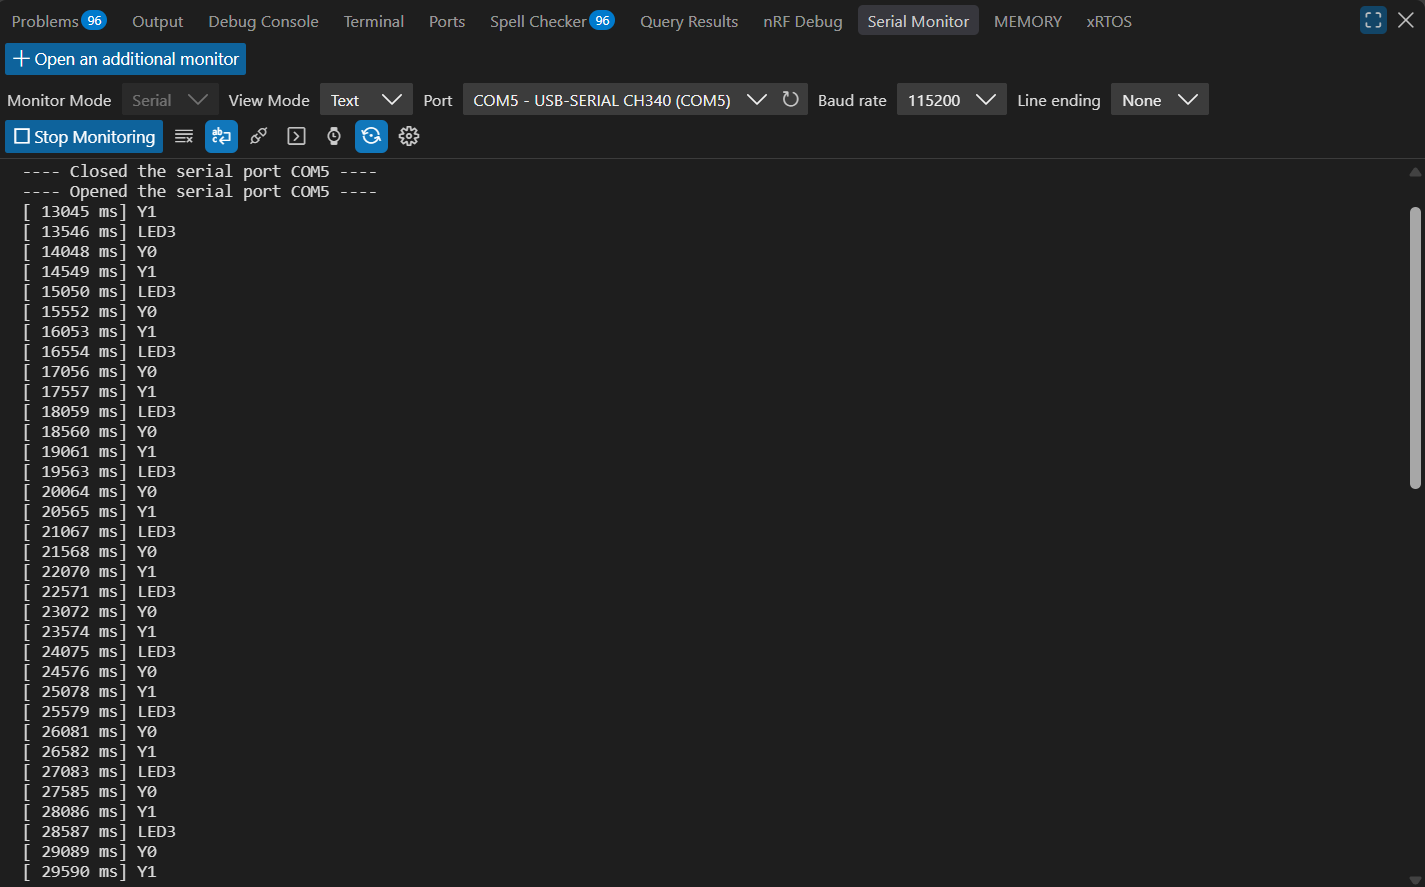
\includegraphics[width=0.92\linewidth]{image/image1.png}
    \caption{Minh chứng log Serial Monitor trên kit thật (115200 baud) - Bài 1}
\end{figure}

\subsubsection{Trả lời câu hỏi bài tập}
\begin{enumerate}[label=(\alph*)]
    \item \textbf{Bạn chọn giá trị ban đầu của ba semaphore như thế nào? Điều gì xảy ra nếu cả ba đều bằng 0? Nếu cả ba đều bằng 1?} \\
    \textbf{Trả lời:}
    \begin{itemize}
        \item \textbf{Cấu hình chọn:} \texttt{sem\_led3 = 1}, \texttt{sem\_y0 = 0}, \texttt{sem\_y1 = 0}. Việc gán \texttt{sem\_led3 = 1} nhằm cấp quyền thực thi đầu tiên cho \texttt{thread\_led3} ngay khi khởi động, trong khi hai luồng còn lại chuyển sang trạng thái blocked chờ lượt từ luồng trước đó.
        \item \textbf{Nếu cả ba đều bằng 0:} Xảy ra hiện tượng \textbf{Deadlock} (khóa chết hệ thống). Cả ba luồng khi khởi động đều gọi \texttt{k\_sem\_take} và lập tức bị chuyển sang trạng thái BLOCKED vĩnh viễn vì không có luồng nào được cấp vé ban đầu. Kết quả là hệ thống đứng im, không có đèn nào sáng.
        \item \textbf{Nếu cả ba đều bằng 1:} Cả ba luồng đều vượt qua lệnh \texttt{k\_sem\_take} ngay lập tức ở lần chạy đầu tiên. Khi đó cả ba đèn LED3, Y0, Y1 sẽ cùng bật sáng đồng thời trong 500 ms đầu, vi phạm hoàn toàn yêu cầu của đề bài là "không bao giờ có hai đèn cùng sáng".
    \end{itemize}
    
    \item \textbf{Muốn đổi thứ tự thành LED3 $\rightarrow$ Y1 $\rightarrow$ Y0, bạn phải sửa những gì?} \\
    \textbf{Trả lời:} 
	
	Ta chỉ cần sửa đối tượng semaphore được giải phóng trong lệnh \texttt{k\_sem\_give} ở cuối mỗi hàm luồng:
    \begin{itemize}
        \item Trong \texttt{fn\_thread\_led3}: Sửa \texttt{k\_sem\_give(\&sem\_y0)} thành \texttt{k\_sem\_give(\&sem\_y1)} (chuyền lượt cho Y1).
        \item Trong \texttt{fn\_thread\_y1}: Sửa \texttt{k\_sem\_give(\&sem\_led3)} thành \texttt{k\_sem\_give(\&sem\_y0)} (chuyền lượt cho Y0).
        \item Trong \texttt{fn\_thread\_y0}: Sửa \texttt{k\_sem\_give(\&sem\_y1)} thành \texttt{k\_sem\_give(\&sem\_led3)} (chuyền ngược về LED3 để khép kín chu trình).
    \end{itemize}
    \textit{Lưu ý:} Giá trị khởi tạo ban đầu vẫn giữ: \texttt{sem\_led3 = 1}, \texttt{sem\_y1 = 0}, \texttt{sem\_y0 = 0}.
\end{enumerate}

\newpage
% =============================================================================
% BÀI 2
% =============================================================================
\subsection{Bài 2: Giám sát tín hiệu có Timeout}

\begin{tcolorbox}[
    enhanced, colback=black!2, colframe=black!60, boxrule=1pt, arc=2.5mm, drop shadow,
    attach boxed title to top left={xshift=4mm, yshift=-3mm},
    boxed title style={enhanced, colback=black!85, colframe=black!85, boxrule=1pt, arc=2.5mm, drop shadow, left=6pt, right=6pt, top=2pt, bottom=2pt},
    title=\textcolor{white}{\large\textbf{Yêu cầu đề bài (Trích phiếu bài tập)}}
]
\bfseries
\vspace{0.2cm}
\begin{itemize}
    \item Tạo một \texttt{k\_timer} chạy chế độ one-shot; trong callback (ISR), sau khi \texttt{k\_sem\_give(\&sig\_sem)}, tự khởi động lại timer với chu kỳ lần lượt 1 s, 1 s, 4 s rồi lặp lại (mô phỏng tín hiệu thỉnh thoảng bị mất).
    \item Thread \texttt{thread\_monitor} chờ tín hiệu bằng \texttt{k\_sem\_take(\&sig\_sem, K\_MSEC(2000))} và kiểm tra giá trị trả về:
    \begin{itemize}
        \item \texttt{0} $\rightarrow$ in \texttt{Nhan tin hieu}, nháy Y0 hai lần (mỗi lần 100 ms sáng / 100 ms tắt).
        \item \texttt{-EAGAIN} $\rightarrow$ in \texttt{TIMEOUT - mat tin hieu!} và đảo trạng thái LED3.
    \end{itemize}
    \item ISR không được in log, không điều khiển đèn — chỉ give và khởi động lại timer.
\end{itemize}
\end{tcolorbox}

\vspace{0.3cm}
\subsubsection{Mã nguồn chương trình (\texttt{src/main.c})}
\begin{lstlisting}[language=C]
#include <stdio.h>
#include <errno.h>
#include <zephyr/kernel.h>
#include <zephyr/drivers/gpio.h>

#define LED0_NODE DT_ALIAS(led0) /* LED3 - PE4: Den canh bao Timeout */
#define LED1_NODE DT_ALIAS(led1) /* Y0   - PE5: Den bao nhan tin hieu */

static const struct gpio_dt_spec led3 = GPIO_DT_SPEC_GET(LED0_NODE, gpios);
static const struct gpio_dt_spec y0   = GPIO_DT_SPEC_GET(LED1_NODE, gpios);

/* Khoi tao Binary Semaphore: ban dau = 0, toi da = 1 */
K_SEM_DEFINE(sig_sem, 0, 1);

static const int delay_pattern_ms[] = {1000, 1000, 4000};
static int pattern_idx = 0;

/* ISR cua Timer: Chi give semaphore va khoi dong lai timer, khong goi printf/sleep */
static void sig_timer_isr(struct k_timer *timer)
{
	k_sem_give(&sig_sem);
	k_timer_start(timer, K_MSEC(delay_pattern_ms[pattern_idx]), K_NO_WAIT);
	pattern_idx = (pattern_idx + 1) % 3;
}
K_TIMER_DEFINE(sig_timer, sig_timer_isr, NULL);

/* Thread giam sat tin hieu */
void fn_thread_monitor(void *p1, void *p2, void *p3)
{
	gpio_pin_configure_dt(&led3, GPIO_OUTPUT_INACTIVE);
	gpio_pin_configure_dt(&y0,   GPIO_OUTPUT_INACTIVE);

	while (1) {
		int ret = k_sem_take(&sig_sem, K_MSEC(2000));

		if (ret == 0) {
			/* Nhan tin hieu thanh cong: nhay Y0 hai lan (100ms sang / 100ms tat) */
			printf("[%6u ms] Nhan tin hieu\n", k_uptime_get_32());
			for (int i = 0; i < 2; i++) {
				gpio_pin_set_dt(&y0, 1);
				k_msleep(100);
				gpio_pin_set_dt(&y0, 0);
				k_msleep(100);
			}
		} else if (ret == -EAGAIN) {
			/* Qua 2000 ms khong co tin hieu: Bao TIMEOUT va dao LED3 */
			printf("[%6u ms] TIMEOUT - mat tin hieu!\n", k_uptime_get_32());
			gpio_pin_toggle_dt(&led3);
		}
	}
}

K_THREAD_DEFINE(thread_monitor, 1024, fn_thread_monitor, NULL, NULL, NULL, 5, 0, 0);

int main(void)
{
	printf("=== BKIT ARM4: Lab 2 - Bai 2: Giam sat tin hieu co Timeout ===\n");
	k_timer_start(&sig_timer, K_MSEC(delay_pattern_ms[0]), K_NO_WAIT);
	pattern_idx = 1;
	return 0;
}
\end{lstlisting}

\subsubsection{Kết quả thực nghiệm \& Log Serial Monitor}
\begin{lstlisting}[basicstyle=\ttfamily\scriptsize]
=== BKIT ARM4: Lab 2 - Bai 2: Giam sat tin hieu co Timeout ===
[  1000 ms] Nhan tin hieu
[  2400 ms] Nhan tin hieu
[  4800 ms] TIMEOUT - mat tin hieu!
[  6800 ms] Nhan tin hieu
[  8200 ms] Nhan tin hieu
[ 10600 ms] TIMEOUT - mat tin hieu!
[ 12600 ms] Nhan tin hieu
[ 14000 ms] Nhan tin hieu
[ 16400 ms] TIMEOUT - mat tin hieu!
\end{lstlisting}

\begin{figure}[H]
    \centering
    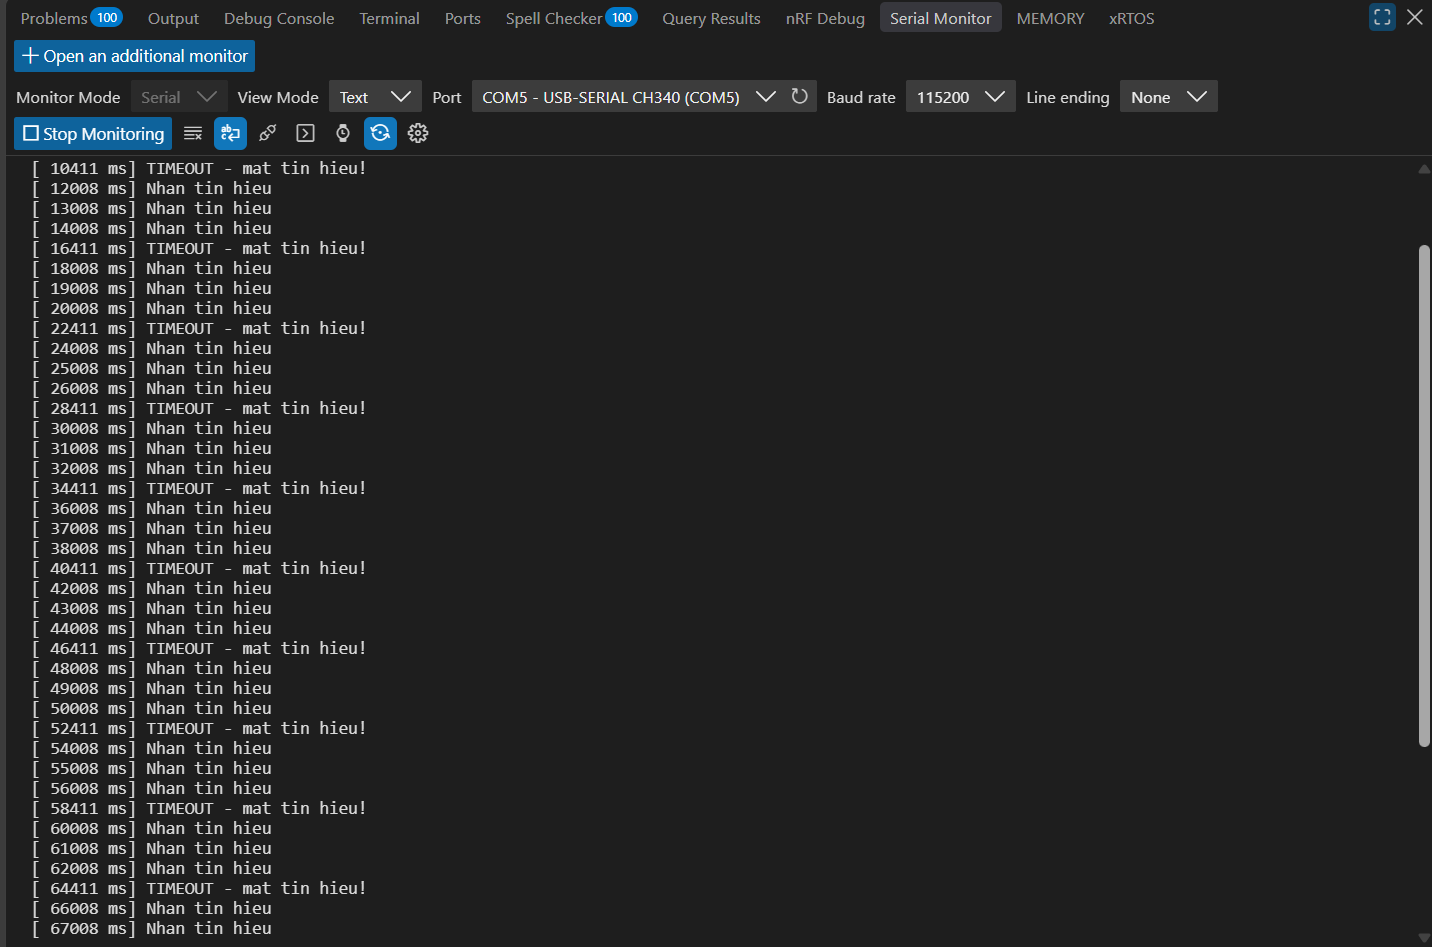
\includegraphics[width=0.92\linewidth]{image/image2.png}
    \caption{Minh chứng log Serial Monitor trên kit thật (115200 baud) - Bài 2}
\end{figure}

\subsubsection{Trả lời câu hỏi bài tập}
\begin{enumerate}[label=(\alph*)]
    \item \textbf{Trong log, mỗi chu kỳ 6 s có bao nhiêu lần timeout và tại thời điểm nào? Giải thích con số đó.} \\
    \textbf{Trả lời:}
    \begin{itemize}
        \item \textbf{Số lần timeout:} Mỗi chu kỳ 6s của timer ($1\text{s} + 1\text{s} + 4\text{s} = 6\text{s}$) có \textbf{đúng 1 lần timeout}.
        \item \textbf{Thời điểm \& Giải thích:} Sau 2 lần nhận tín hiệu đầu tiên (khoảng cách 1s, nhỏ hơn timeout 2s nên nhận thành công), timer được nạp chu kỳ one-shot là 4000 ms. Luồng \texttt{thread\_monitor} gọi \texttt{k\_sem\_take} với thời gian chờ tối đa 2000 ms (\texttt{K\_MSEC(2000)}). Khi chờ đủ 2000 ms mà vẫn chưa có tín hiệu từ timer, hàm \texttt{k\_sem\_take} hết hạn và trả về mã lỗi \texttt{-EAGAIN} $\rightarrow$ Luồng ghi nhận TIMEOUT và đảo trạng thái LED3. Tại giây thứ 4 của khoảng chờ, timer mới hết hạn và gọi \texttt{k\_sem\_give(\&sig\_sem)}. Tín hiệu này được lưu lại trong semaphore để luồng nhận ngay ở chu kỳ tiếp theo.
    \end{itemize}
    
    \item \textbf{Vì sao ISR không được gọi \texttt{k\_sem\_take(\&sig\_sem, K\_FOREVER)} hay \texttt{k\_msleep()}?} \\
    \item 
    \textbf{Trả lời:} 
	ISR (trình phục vụ ngắt) chạy trong ngữ cảnh ngắt phần cứng, không phải là một luồng (thread) có không gian ngăn xếp (stack) riêng của bộ lập lịch RTOS, nên nó \textbf{không thể bị chuyển sang trạng thái ngủ/chờ (BLOCKED/SLEEP)}. Nếu gọi hàm chờ như \texttt{k\_sem\_take(..., K\_FOREVER)} hoặc \texttt{k\_msleep()} trong ISR, nhân hệ điều hành Zephyr sẽ phát hiện vi phạm và kích hoạt Kernel Panic / Fatal Usage Fault (báo lỗi: \textit{"Illegal use of wait in ISR context"}), dẫn đến việc khóa cứng CPU và treo toàn bộ hệ thống ngay lập tức. ISR phải thực thi với tốc độ cực nhanh và thoát ngay để CPU tiếp nhận các ngắt khác.
    
    \item \textbf{Nếu ISR give hai lần liên tiếp trước khi thread kịp take thì thread xử lý mấy lần? Muốn không mất lần nào thì sửa khai báo semaphore ra sao?} \\
    \textbf{Trả lời:}
    \begin{itemize}
        \item \textbf{Số lần xử lý:} Thread chỉ xử lý \textbf{đúng 1 lần}, lần give thứ hai bị mất hoàn toàn. Do \texttt{sig\_sem} được khai báo là Binary Semaphore với giới hạn tối đa \texttt{limit = 1}. Khi semaphore đã đạt giá trị 1 mà thread chưa kịp lấy, mọi lệnh \texttt{k\_sem\_give} tiếp theo sẽ không làm tăng bộ đếm mà bị bỏ qua.
        \item \textbf{Cách sửa:} Chuyển sang dùng Counting Semaphore bằng cách tăng tham số giới hạn tối đa (\texttt{limit}) đủ lớn, ví dụ: \texttt{K\_SEM\_DEFINE(sig\_sem, 0, 10);}. Khi đó bộ đếm semaphore có thể tích lũy nhiều lần give liên tiếp để thread lấy dần ra xử lý mà không bị mất.
    \end{itemize}
\end{enumerate}

% =============================================================================
% BÀI 3
% =============================================================================
\subsection{Bài 3: Chia sẻ 2 kênh output cho 4 worker bằng Counting Semaphore}

\begin{tcolorbox}[
    enhanced, colback=black!2, colframe=black!60, boxrule=1pt, arc=2.5mm, drop shadow,
    attach boxed title to top left={xshift=4mm, yshift=-3mm},
    boxed title style={enhanced, colback=black!85, colframe=black!85, boxrule=1pt, arc=2.5mm, drop shadow, left=6pt, right=6pt, top=2pt, bottom=2pt},
    title=\textcolor{white}{\large\textbf{Yêu cầu đề bài (Trích phiếu bài tập)}}
]
\bfseries
\vspace{0.2cm}
\begin{itemize}
    \item Hệ thống có 2 kênh output: Y0 và Y1. Có 4 worker muốn dùng kênh, mỗi worker lặp vô hạn: xin một kênh trống $\rightarrow$ bật đèn kênh đó trong thời gian làm việc $\rightarrow$ tắt đèn, trả kênh $\rightarrow$ nghỉ.
    \item Thông số Worker: W1 (làm 1000ms / nghỉ 500ms), W2 (1500ms / 700ms), W3 (2000ms / 300ms), W4 (2500ms / 900ms).
    \item Dùng một hàm thread \texttt{thread\_worker} nhận cấu hình qua \texttt{p1}, tạo 4 lần \texttt{K\_THREAD\_DEFINE}.
    \item Dùng \texttt{K\_SEM\_DEFINE(pool\_sem, 2, 2)} giới hạn tối đa 2 worker đồng thời, và một Mutex bảo vệ mảng trạng thái \texttt{ch\_busy[2]}.
    \item LED3 sáng khi không còn kênh trống (\texttt{k\_sem\_count\_get == 0}), tắt khi có kênh trống.
    \item In log mỗi lần lấy/trả kênh: \texttt{[t] W2 dung kenh Y1 / [t] W2 tra kenh Y1}.
\end{itemize}
\end{tcolorbox}

\vspace{0.3cm}
\subsubsection{Mã nguồn chương trình (\texttt{src/main.c})}
\begin{lstlisting}[language=C]
#include <stdio.h>
#include <stdbool.h>
#include <zephyr/kernel.h>
#include <zephyr/drivers/gpio.h>

#define LED0_NODE DT_ALIAS(led0) /* LED3 - PE4: Bao ca 2 kenh deu ban */
#define LED1_NODE DT_ALIAS(led1) /* Y0   - PE5: Kenh output 0 */
#define LED2_NODE DT_ALIAS(led2) /* Y1   - PE6: Kenh output 1 */

static const struct gpio_dt_spec led3 = GPIO_DT_SPEC_GET(LED0_NODE, gpios);
static const struct gpio_dt_spec channels[2] = {
	GPIO_DT_SPEC_GET(LED1_NODE, gpios),
	GPIO_DT_SPEC_GET(LED2_NODE, gpios)
};
static const char *const ch_names[2] = {"Y0", "Y1"};

/* Counting semaphore gioi han 2 kenh; Mutex bao ve mang trang thai kenh */
K_SEM_DEFINE(pool_sem, 2, 2);
K_MUTEX_DEFINE(ch_mutex);

static bool ch_busy[2] = {false, false};

struct worker_cfg {
	int id;
	int work_ms;
	int rest_ms;
};

static const struct worker_cfg cfg1 = {1, 1000, 500};
static const struct worker_cfg cfg2 = {2, 1500, 700};
static const struct worker_cfg cfg3 = {3, 2000, 300};
static const struct worker_cfg cfg4 = {4, 2500, 900};

void thread_worker(void *p1, void *p2, void *p3)
{
	const struct worker_cfg *cfg = (const struct worker_cfg *)p1;

	while (1) {
		/* 1. Xin ve tu Counting Semaphore */
		k_sem_take(&pool_sem, K_FOREVER);

		/* 2. Chon kenh trong duoc bao ve boi Mutex */
		k_mutex_lock(&ch_mutex, K_FOREVER);
		int ch = -1;
		if (!ch_busy[0]) {
			ch = 0;
			ch_busy[0] = true;
		} else if (!ch_busy[1]) {
			ch = 1;
			ch_busy[1] = true;
		}
		if (k_sem_count_get(&pool_sem) == 0) {
			gpio_pin_set_dt(&led3, 1);
		}
		k_mutex_unlock(&ch_mutex);

		/* 3. Dung kenh lam viec */
		printf("[%6u ms] W%d dung kenh %s\n", k_uptime_get_32(), cfg->id, ch_names[ch]);
		gpio_pin_set_dt(&channels[ch], 1);
		k_msleep(cfg->work_ms);
		gpio_pin_set_dt(&channels[ch], 0);

		/* 4. Tra kenh an toan qua Mutex */
		printf("[%6u ms] W%d tra kenh %s\n", k_uptime_get_32(), cfg->id, ch_names[ch]);
		k_mutex_lock(&ch_mutex, K_FOREVER);
		ch_busy[ch] = false;
		gpio_pin_set_dt(&led3, 0);
		k_mutex_unlock(&ch_mutex);

		k_sem_give(&pool_sem);

		/* 5. Nghi ngoi */
		k_msleep(cfg->rest_ms);
	}
}

K_THREAD_DEFINE(worker1, 1024, thread_worker, (void *)&cfg1, NULL, NULL, 5, 0, 0);
K_THREAD_DEFINE(worker2, 1024, thread_worker, (void *)&cfg2, NULL, NULL, 5, 0, 0);
K_THREAD_DEFINE(worker3, 1024, thread_worker, (void *)&cfg3, NULL, NULL, 5, 0, 0);
K_THREAD_DEFINE(worker4, 1024, thread_worker, (void *)&cfg4, NULL, NULL, 5, 0, 0);

int main(void)
{
	gpio_pin_configure_dt(&led3, GPIO_OUTPUT_INACTIVE);
	gpio_pin_configure_dt(&channels[0], GPIO_OUTPUT_INACTIVE);
	gpio_pin_configure_dt(&channels[1], GPIO_OUTPUT_INACTIVE);
	printf("=== BKIT ARM4: Lab 2 - Bai 3: Chia se 2 kenh output cho 4 worker ===\n");
	return 0;
}
\end{lstlisting}

\subsubsection{Kết quả thực nghiệm \& Log Serial Monitor}
\begin{lstlisting}[basicstyle=\ttfamily\scriptsize]
=== BKIT ARM4: Lab 2 - Bai 3: Chia se 2 kenh output cho 4 worker ===
[     0 ms] W1 dung kenh Y0
[     0 ms] W2 dung kenh Y1
[  1000 ms] W1 tra kenh Y0
[  1000 ms] W3 dung kenh Y0
[  1500 ms] W2 tra kenh Y1
[  1500 ms] W4 dung kenh Y1
[  3000 ms] W3 tra kenh Y0
[  3000 ms] W1 dung kenh Y0
[  4000 ms] W1 tra kenh Y0
[  4000 ms] W4 tra kenh Y1
[  4000 ms] W2 dung kenh Y0
[  4000 ms] W3 dung kenh Y1
[  5500 ms] W2 tra kenh Y0
[  5500 ms] W1 dung kenh Y0
[  6000 ms] W3 tra kenh Y1
[  6000 ms] W4 dung kenh Y1
\end{lstlisting}

\begin{figure}[H]
    \centering
    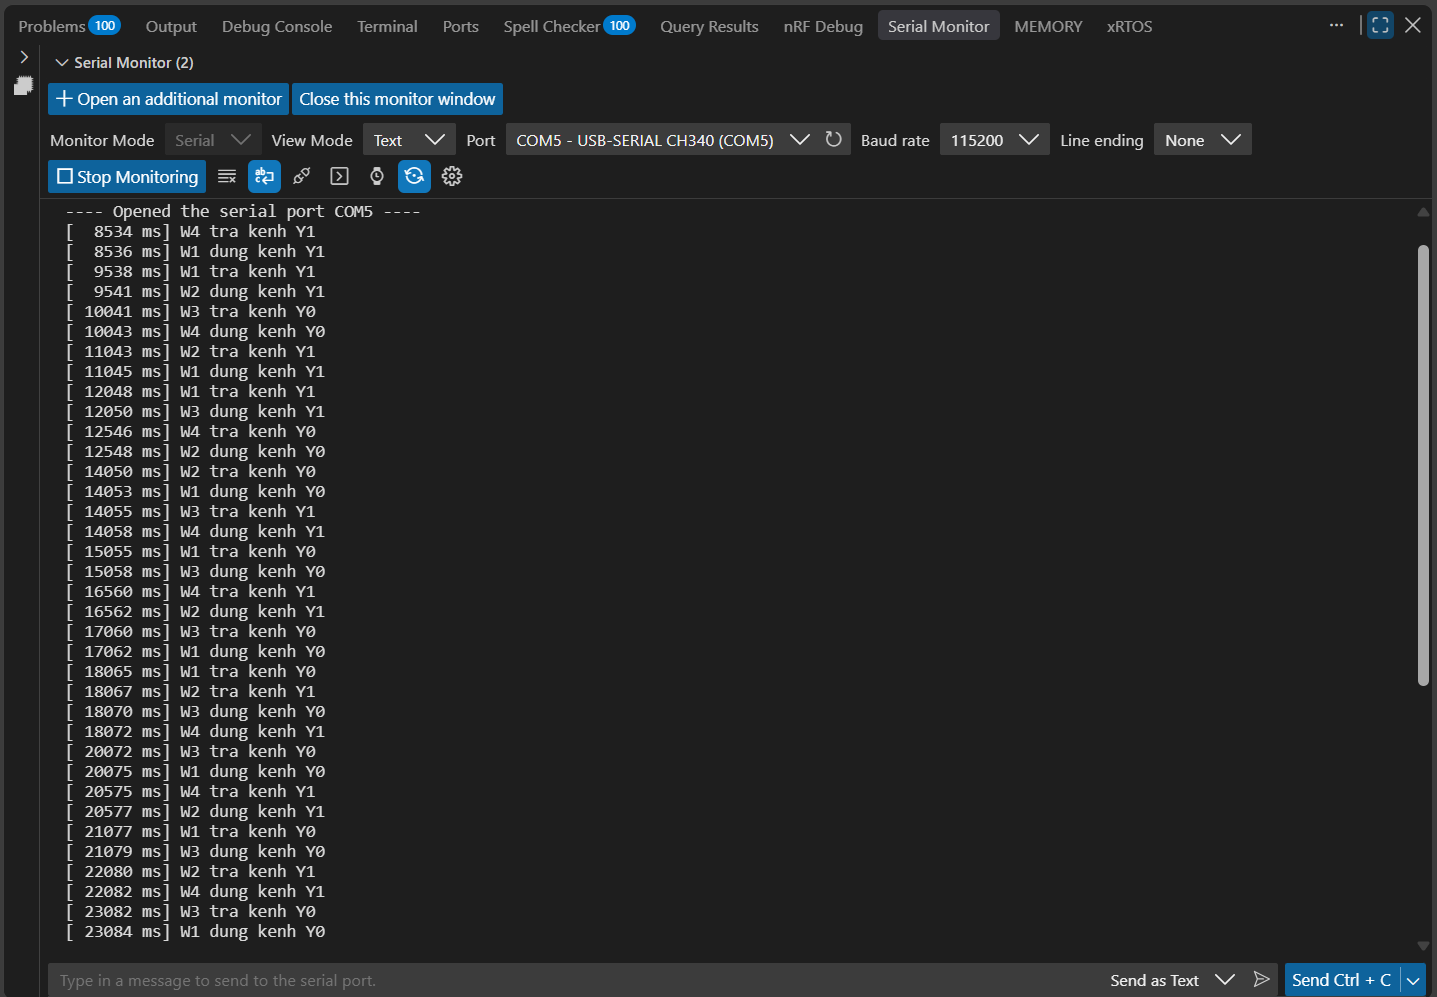
\includegraphics[width=0.92\linewidth]{image/image3.png}
    \caption{Minh chứng log Serial Monitor trên kit thật (115200 baud) - Bài 3}
\end{figure}

\subsubsection{Trả lời câu hỏi bài tập}
\begin{enumerate}[label=(\alph*)]
    \item \textbf{Vì sao cần cả counting semaphore và mutex? Mỗi cái giải quyết vấn đề gì?} \\
    \textbf{Trả lời:}
    \begin{itemize}
        \item \textbf{Counting Semaphore (\texttt{pool\_sem = 2}):} Giải quyết bài toán \textbf{định lượng và giới hạn tài nguyên} (Resource Capacity Control). Giới hạn tối đa 2 worker được phép sử dụng kênh đồng thời. Khi cả 2 kênh đều bận (\texttt{count == 0}), semaphore tự động đưa worker thứ 3 và thứ 4 vào hàng đợi chờ (BLOCKED) mà không tiêu tốn chu kỳ CPU. Nhược điểm: Semaphore chỉ đếm số lượng tài nguyên còn trống chứ không chỉ ra cụ thể kênh nào (kênh 0 hay kênh 1) đang rảnh.
        \item \textbf{Mutex (\texttt{ch\_mutex}):} Giải quyết bài toán \textbf{loại trừ tương hỗ} (Mutual Exclusion) cho bảng trạng thái \texttt{ch\_busy[2]}. Đảm bảo việc kiểm tra và cập nhật mảng trạng thái (tìm kênh rảnh và đánh dấu bận) diễn ra nguyên tử (Critical Section), ngăn chặn tranh chấp giữa các worker.
    \end{itemize}
    
    \item \textbf{Nếu thay \texttt{pool\_sem} bằng binary semaphore thì hệ thống chạy thế nào? Nếu bỏ mutex thì lỗi gì có thể xảy ra?} \\
    \textbf{Trả lời:}
    \begin{itemize}
        \item \textbf{Nếu thay \texttt{pool\_sem} bằng Binary Semaphore (\texttt{initial = 1, max = 1}):} Giới hạn tài nguyên bị giảm từ 2 xuống 1. Tại mọi thời điểm chỉ có DUY NHẤT 1 worker được làm việc, kênh output còn lại bị bỏ phí hoàn toàn. Thời gian chờ đợi của các worker tăng gấp đôi và hiệu năng hệ thống giảm một nửa.
        \item \textbf{Nếu bỏ Mutex:} Xảy ra lỗi Race Condition (tranh chấp điều kiện) trên mảng \texttt{ch\_busy[2]}. Nếu 2 worker cùng thức dậy và kiểm tra \texttt{ch\_busy[0] == false} trước khi kịp gán \texttt{true}, \textbf{cả hai worker sẽ cùng chọn và điều khiển chung kênh Y0}! Khi đó kênh Y1 bị bỏ trống vô cớ, còn đèn Y0 bị 2 worker bật tắt chồng chéo gây loạn logic.
    \end{itemize}
    
    \item \textbf{Từ log, có lúc nào cả 4 worker cùng chờ không? Worker nào chờ lâu nhất?} \\
    \textbf{Trả lời:}
    \begin{itemize}
        \item \textbf{Có lúc nào cả 4 worker cùng chờ không?} \textbf{Không bao giờ}. Vì điều kiện để một worker phải chờ là số vé trong \texttt{pool\_sem} bằng 0, đồng nghĩa với việc đang có đúng 2 worker đang chiếm kênh làm việc. Do đó, tối đa chỉ có 2 worker rơi vào trạng thái chờ (BLOCKED) cùng một lúc.
        \item \textbf{Worker nào chờ lâu nhất?} \textbf{Worker 4 (W4)} là worker phải chờ lâu nhất. Do W4 có thời gian làm việc dài nhất (2500 ms) và thời gian nghỉ cũng dài (900 ms). Khi W4 nghỉ xong và quay lại xin kênh, các worker có chu kỳ làm việc và thời gian nghỉ ngắn hơn (như W3 chỉ nghỉ 300 ms, W1 nghỉ 500 ms) đã nhanh chân chiếm mất các kênh vừa rảnh, khiến W4 có thời gian tích lũy chờ đợi lâu nhất giữa các lần được cấp kênh.
    \end{itemize}
\end{enumerate}

\newpage
% =============================================================================
% BÀI 4
% =============================================================================
\subsection{Bài 4: Thu thập dữ liệu từ ISR qua Message Queue}

\begin{tcolorbox}[
    enhanced, colback=black!2, colframe=black!60, boxrule=1pt, arc=2.5mm, drop shadow,
    attach boxed title to top left={xshift=4mm, yshift=-3mm},
    boxed title style={enhanced, colback=black!85, colframe=black!85, boxrule=1pt, arc=2.5mm, drop shadow, left=6pt, right=6pt, top=2pt, bottom=2pt},
    title=\textcolor{white}{\large\textbf{Yêu cầu đề bài (Trích phiếu bài tập)}}
]
\bfseries
\vspace{0.2cm}
\begin{itemize}
    \item Định nghĩa \texttt{struct sample \{ uint32\_t seq; uint32\_t t\_ms; \};} và hàng đợi \texttt{K\_MSGQ\_DEFINE(sample\_q, sizeof(struct sample), 8, 4);}.
    \item Một \texttt{k\_timer} chu kỳ 200 ms; trong ISR tạo mẫu (\texttt{seq} tăng dần, \texttt{t\_ms = k\_uptime\_get\_32()}) và gửi bằng \texttt{k\_msgq\_put(..., K\_NO\_WAIT)}. Thất bại $\rightarrow$ tăng \texttt{n\_drop}; thành công $\rightarrow$ tăng \texttt{n\_sent} (dùng \texttt{atomic\_t}).
    \item Thread \texttt{thread\_consumer} lấy từng mẫu và xử lý mất 500 ms (Y0 nháy 250ms sáng / 250ms tắt), tăng \texttt{n\_recv}.
    \item Thread \texttt{thread\_monitor} mỗi 5 s in thống kê gửi/nhận/mất/trong hàng đợi, bật LED3 khi có mẫu bị mất.
    \item \textbf{Phần b}: Giảm thời gian xử lý xuống 150 ms, chạy lại và ghi log chứng minh không còn mẫu bị mất.
\end{itemize}
\end{tcolorbox}

\vspace{0.3cm}
\subsubsection{Mã nguồn chương trình (\texttt{src/main.c})}
\begin{lstlisting}[language=C]
#include <stdio.h>
#include <zephyr/kernel.h>
#include <zephyr/drivers/gpio.h>
#include <zephyr/sys/atomic.h>

#define LED0_NODE DT_ALIAS(led0) /* LED3 - PE4: Bao co mau bi mat */
#define LED1_NODE DT_ALIAS(led1) /* Y0   - PE5: Nhay khi Consumer xu ly mau */

static const struct gpio_dt_spec led3 = GPIO_DT_SPEC_GET(LED0_NODE, gpios);
static const struct gpio_dt_spec y0   = GPIO_DT_SPEC_GET(LED1_NODE, gpios);

struct sample {
	uint32_t seq;
	uint32_t t_ms;
};

/* Message queue tinh: 8 phan tu, can le 4 bytes */
K_MSGQ_DEFINE(sample_q, sizeof(struct sample), 8, 4);

/* Bien dem nguyen tu an toan giua ISR va Thread */
static atomic_t n_sent = ATOMIC_INIT(0);
static atomic_t n_drop = ATOMIC_INIT(0);
static atomic_t n_recv = ATOMIC_INIT(0);

/* Dieu chinh thoi gian xu ly: 500 ms cho Phan a, 150 ms cho Phan b */
#define CONSUME_TIME_MS 150

static void sample_timer_isr(struct k_timer *timer)
{
	static uint32_t current_seq = 0;
	struct sample s;

	current_seq++;
	s.seq = current_seq;
	s.t_ms = k_uptime_get_32();

	/* BAT BUOC dung K_NO_WAIT trong ngat */
	int ret = k_msgq_put(&sample_q, &s, K_NO_WAIT);
	if (ret == 0) {
		atomic_inc(&n_sent);
	} else {
		atomic_inc(&n_drop);
	}
}
K_TIMER_DEFINE(sample_timer, sample_timer_isr, NULL);

/* Thread tieu thu du lieu */
void fn_thread_consumer(void *p1, void *p2, void *p3)
{
	struct sample s;
	gpio_pin_configure_dt(&y0, GPIO_OUTPUT_INACTIVE);

	while (1) {
		k_msgq_get(&sample_q, &s, K_FOREVER);
		atomic_inc(&n_recv);

		gpio_pin_set_dt(&y0, 1);
		k_msleep(CONSUME_TIME_MS / 2);
		gpio_pin_set_dt(&y0, 0);
		k_msleep(CONSUME_TIME_MS / 2);
	}
}

/* Thread giam sat va in thong ke dinh ky 5s */
void fn_thread_monitor(void *p1, void *p2, void *p3)
{
	gpio_pin_configure_dt(&led3, GPIO_OUTPUT_INACTIVE);

	while (1) {
		k_msleep(5000);

		long sent = atomic_get(&n_sent);
		long recv = atomic_get(&n_recv);
		long drop = atomic_get(&n_drop);
		uint32_t in_q = k_msgq_num_used_get(&sample_q);

		printf("[%6u ms] GUI: %ld | NHAN: %ld | MAT: %ld | TRONG HANG DOI: %u/8\n",
		       k_uptime_get_32(), sent, recv, drop, in_q);

		if (drop > 0) {
			gpio_pin_set_dt(&led3, 1);
		}
	}
}

K_THREAD_DEFINE(thread_consumer, 1024, fn_thread_consumer, NULL, NULL, NULL, 5, 0, 0);
K_THREAD_DEFINE(thread_monitor,  1024, fn_thread_monitor,  NULL, NULL, NULL, 6, 0, 0);

int main(void)
{
	printf("=== BKIT ARM4: Lab 2 - Bai 4: Thu thap du lieu tu ISR qua Message Queue ===\n");
	printf("Cau hinh: Chu ky tao mau = 200 ms | Thoi gian xu ly = %d ms\n", CONSUME_TIME_MS);
	k_timer_start(&sample_timer, K_MSEC(200), K_MSEC(200));
	return 0;
}
\end{lstlisting}

\subsubsection{Kết quả thực nghiệm \& Log Serial Monitor}

\noindent\textbf{1. Log Phần a (\texttt{CONSUME\_TIME\_MS = 500} ms — Xảy ra tràn hàng đợi, mất mẫu và LED3 sáng):}
\begin{lstlisting}[basicstyle=\ttfamily\scriptsize]
=== BKIT ARM4: Lab 2 - Bai 4: Thu thap du lieu tu ISR qua Message Queue ===
Cau hinh: Chu ky tao mau = 200 ms | Thoi gian xu ly = 500 ms
[  5000 ms] GUI: 17 | NHAN: 10 | MAT:  7 | TRONG HANG DOI: 7/8
[ 10000 ms] GUI: 18 | NHAN: 20 | MAT: 22 | TRONG HANG DOI: 8/8
[ 15000 ms] GUI: 18 | NHAN: 30 | MAT: 37 | TRONG HANG DOI: 8/8
[ 20000 ms] GUI: 18 | NHAN: 40 | MAT: 52 | TRONG HANG DOI: 8/8
[ 25000 ms] GUI: 18 | NHAN: 50 | MAT: 67 | TRONG HANG DOI: 8/8
\end{lstlisting}

\begin{figure}[H]
    \centering
    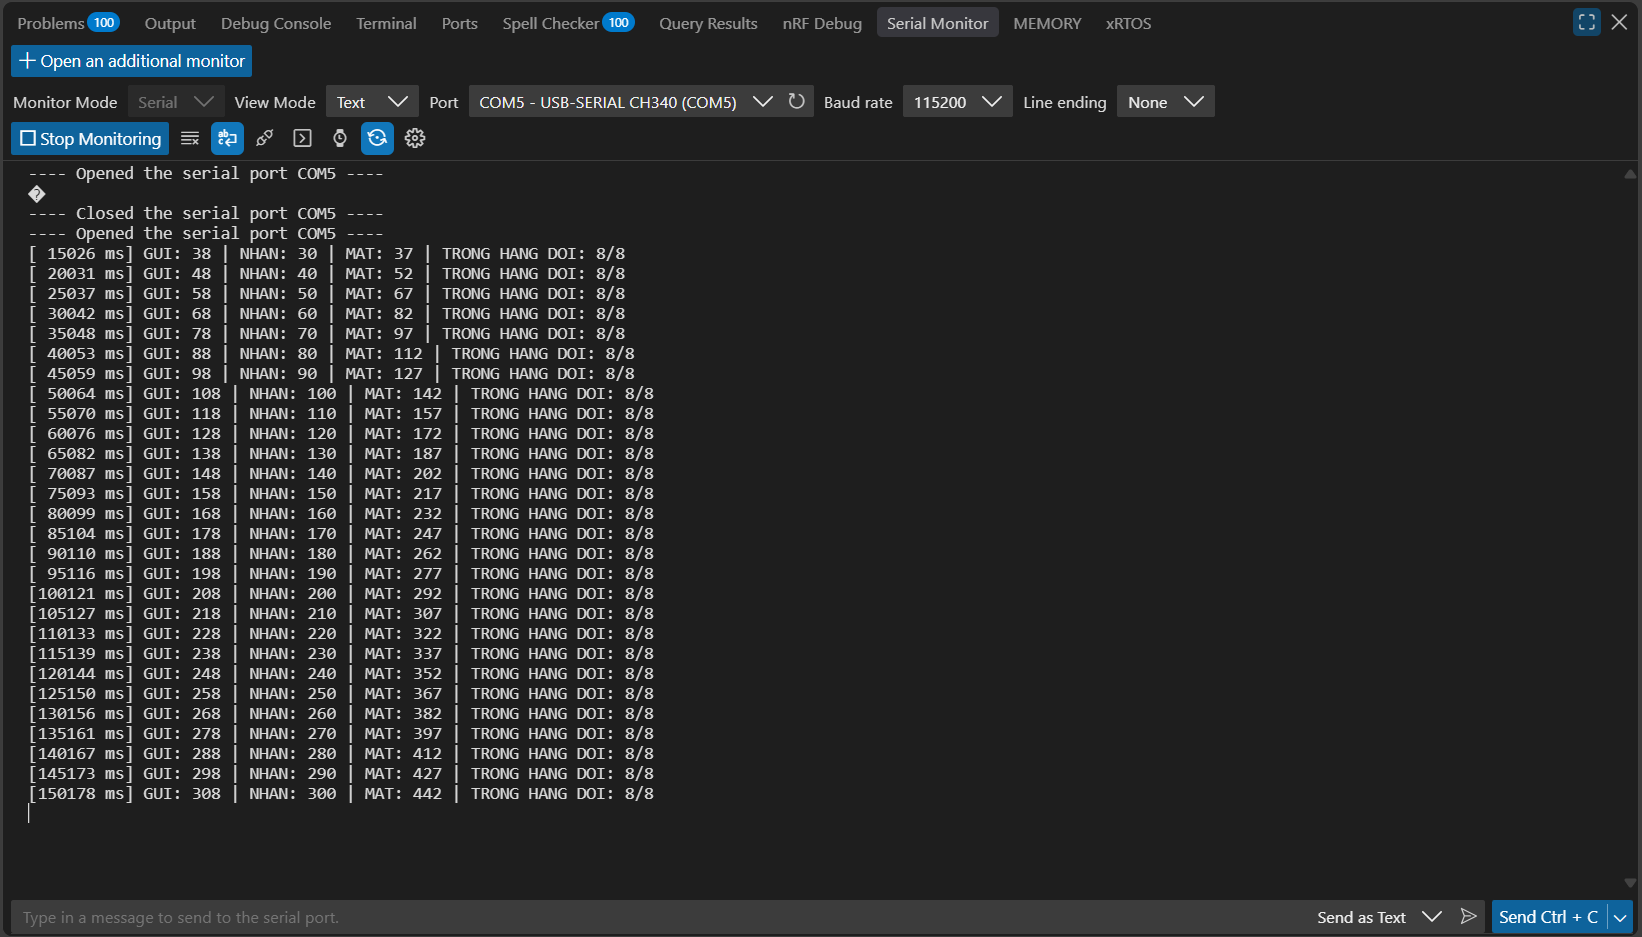
\includegraphics[width=0.92\linewidth]{image/image4.png}
    \caption{Minh chứng log Serial Monitor phần a (Xử lý 500 ms, bị mất mẫu liên tục) - Bài 4}
\end{figure}

\vspace{0.3cm}
\noindent\textbf{2. Log Phần b (\texttt{CONSUME\_TIME\_MS = 150} ms - Cân bằng thông lượng, không mất mẫu nào, LED3 tắt):}
\begin{lstlisting}[basicstyle=\ttfamily\scriptsize]
=== BKIT ARM4: Lab 2 - Bai 4: Thu thap du lieu tu ISR qua Message Queue ===
Cau hinh: Chu ky tao mau = 200 ms | Thoi gian xu ly = 150 ms
[  5000 ms] GUI: 25 | NHAN: 25 | MAT:  0 | TRONG HANG DOI: 0/8
[ 10000 ms] GUI: 50 | NHAN: 50 | MAT:  0 | TRONG HANG DOI: 0/8
[ 15000 ms] GUI: 75 | NHAN: 75 | MAT:  0 | TRONG HANG DOI: 0/8
[ 20000 ms] GUI: 100 | NHAN: 100 | MAT:  0 | TRONG HANG DOI: 0/8
[ 25000 ms] GUI: 125 | NHAN: 125 | MAT:  0 | TRONG HANG DOI: 0/8
\end{lstlisting}

\begin{figure}[H]
    \centering
    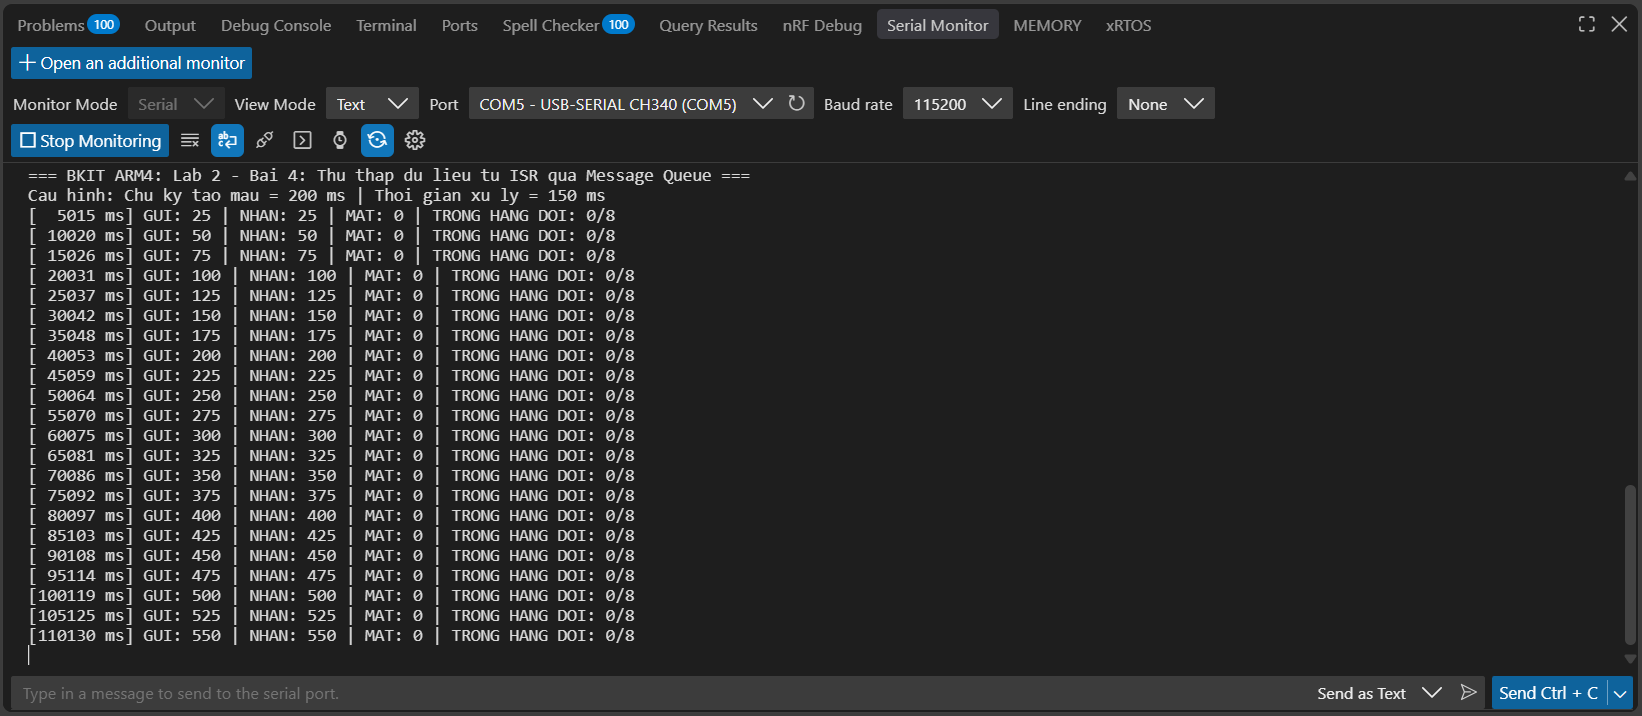
\includegraphics[width=0.92\linewidth]{image/image5.png}
    \caption{Minh chứng log Serial Monitor phần b (Xử lý 150 ms, không mất mẫu nào) - Bài 4}
\end{figure}

\subsubsection{Trả lời câu hỏi bài tập}
\begin{enumerate}[label=(\alph*)]
    \item \textbf{Vì sao trong ISR phải dùng \texttt{K\_NO\_WAIT}? Điều gì sẽ xảy ra nếu dùng \texttt{K\_FOREVER}?} \\
    \textbf{Trả lời:}
    \begin{itemize}
        \item \textbf{Vì sao phải dùng \texttt{K\_NO\_WAIT}:} Trình phục vụ ngắt (ISR) chạy ngoài ngữ cảnh của bất kỳ thread nào, không có cấu trúc quản lý luồng để hệ điều hành đưa vào danh sách chờ ngủ (Wait Queue). ISR bắt buộc phải thực thi ngay và kết thúc tức thì để giải phóng CPU. Vì vậy, khi hàng đợi đầy, ISR buộc phải chấp nhận bỏ mẫu (drop) bằng tham số \texttt{K\_NO\_WAIT} chứ không được phép dừng lại chờ.
        \item \textbf{Điều gì sẽ xảy ra nếu dùng \texttt{K\_FOREVER}:} Nhân hệ điều hành Zephyr sẽ kích hoạt Fatal Exception / Kernel Panic ngay lập tức (thông báo lỗi: \textit{"Illegal use of wait in ISR context!"}), dẫn đến việc dừng hoạt động và khóa cứng CPU (halt system).
    \end{itemize}
    
    \item \textbf{Với tốc độ phần a, tính lý thuyết: mỗi giây có bao nhiêu mẫu bị mất khi hàng đợi đã đầy? So sánh với log.} \\
    \textbf{Trả lời:}
    \begin{itemize}
        \item \textbf{Tính toán lý thuyết:}
        \begin{itemize}
            \item Tốc độ sinh mẫu của Timer ISR: $1000\text{ ms} / 200\text{ ms} = 5\text{ mẫu / giây}$.
            \item Tốc độ tiêu thụ tối đa của Consumer (xử lý 500 ms): $1000\text{ ms} / 500\text{ ms} = 2\text{ mẫu / giây}$.
            \item Khi hàng đợi 8 phần tử đã đầy, mỗi giây lượng mẫu dôi dư không thể chứa vào hàng đợi là:
            $$5 - 2 = 3\text{ mẫu bị mất mỗi giây.}$$
        \end{itemize}
        \item \textbf{So sánh với thực tế trên log:}
        \begin{itemize}
            \item Thread monitor in thống kê mỗi 5 giây (5000 ms).
            \item Trên log, số mẫu mất sau mỗi khoảng 5 giây tăng đều đặn thêm: $5\text{ giây} \times 3\text{ mẫu/giây} = \mathbf{15\text{ mẫu}}$ (các mốc MAT tăng từ $7 \rightarrow 22 \rightarrow 37 \rightarrow 52 \rightarrow 67$).
            \item \textbf{Kết luận:} Số liệu thực tế trên log Serial Monitor khớp hoàn toàn 100\% với tính toán lý thuyết ($15\text{ mẫu} / 5\text{s} = 3\text{ mẫu/s}$).
        \end{itemize}
    \end{itemize}
    
    \item \textbf{Tăng kích thước hàng đợi từ 8 lên 64 có giải quyết được vấn đề ở phần a không? Vì sao?} \\
    \textbf{Trả lời:}
    \begin{itemize}
        \item \textbf{Không giải quyết được vấn đề.}
        \item \textbf{Giải thích:} Việc tăng kích thước hàng đợi lên 64 chỉ làm \textbf{trì hoãn thời điểm bắt đầu mất mẫu}, chứ không ngăn chặn được việc mất mẫu. Do tốc độ sinh mẫu ($5\text{ mẫu/s}$) luôn lớn hơn tốc độ tiêu thụ ($2\text{ mẫu/s}$), lượng mẫu tích tụ liên tục với tốc độ $3\text{ mẫu/s}$. Với dung lượng 64 mẫu, hàng đợi sẽ đầy kín sau:
        $$t_{full} = \frac{64}{3} \approx 21.3\text{ giây.}$$
        Sau giây thứ 21.3, khi 64 ô đã đầy, hệ thống vẫn tiếp tục làm rơi 3 mẫu mỗi giây như trước và LED3 lại bật sáng. Biện pháp duy nhất giải quyết triệt để là tối ưu hóa Consumer để tốc độ xử lý nhanh hơn tốc độ sinh mẫu (thời gian xử lý $< 200\text{ ms}$, như đã chứng minh ở Phần b với 150 ms).
    \end{itemize}
\end{enumerate}

% =============================================================================
% BÀI 5
% =============================================================================
\subsection{Bài 5: Đèn giao thông có nút xin qua đường (Bài tổng hợp)}

\begin{tcolorbox}[
    enhanced, colback=black!2, colframe=black!60, boxrule=1pt, arc=2.5mm, drop shadow,
    attach boxed title to top left={xshift=4mm, yshift=-3mm},
    boxed title style={enhanced, colback=black!85, colframe=black!85, boxrule=1pt, arc=2.5mm, drop shadow, left=6pt, right=6pt, top=2pt, bottom=2pt},
    title=\textcolor{white}{\large\textbf{Yêu cầu đề bài (Trích phiếu bài tập)}}
]
\bfseries
\vspace{0.2cm}
\begin{itemize}
    \item Thread \texttt{thread\_traffic\_light} điều khiển: Y0 = ĐỎ, Y1 = XANH, cả hai = VÀNG; chu kỳ ĐỎ 7 s $\rightarrow$ XANH 5 s $\rightarrow$ VÀNG 2 s.
    \item Nút xin qua đường giả lập bằng \texttt{k\_timer} one-shot: lần đầu ở giây thứ 10, sau đó cách nhau 14 s, 8 s, 17 s. ISR give semaphore \texttt{ped\_sem}.
    \item Quy tắc ưu tiên người đi bộ: Đèn XANH luôn sáng ít nhất 2 s. Sau 2 s, hủy yêu cầu cũ (\texttt{k\_sem\_reset}), rồi chờ yêu cầu mới bằng \texttt{k\_sem\_take(\&ped\_sem, thời\_gian\_xanh\_còn\_lại)}. Nếu có yêu cầu thì kết thúc pha XANH ngay và chuyển sang VÀNG. Yêu cầu đến lúc ĐỎ hoặc VÀNG không có tác dụng.
    \item \textbf{Ghi log tập trung}: Duy nhất thread \texttt{thread\_logger} (độ ưu tiên thấp nhất - 10) được gọi \texttt{printf}. Các luồng và ISR gửi sự kiện \texttt{struct evt \{ type, phase, t\_ms \}} vào \texttt{log\_q} bằng \texttt{K\_NO\_WAIT}.
    \item Thread \texttt{thread\_led\_blinky} (ưu tiên 7): LED3 nháy 1 s sáng / 1 s tắt báo Heartbeat hệ thống.
\end{itemize}
\end{tcolorbox}

\vspace{0.3cm}
\subsubsection{Mã nguồn chương trình (\texttt{src/main.c})}
\begin{lstlisting}[language=C]
#include <stdio.h>
#include <errno.h>
#include <zephyr/kernel.h>
#include <zephyr/drivers/gpio.h>

#define LED0_NODE DT_ALIAS(led0) /* LED3 - PE4: Heartbeat */
#define LED1_NODE DT_ALIAS(led1) /* Y0   - PE5: Den DO */
#define LED2_NODE DT_ALIAS(led2) /* Y1   - PE6: Den XANH */

static const struct gpio_dt_spec led3 = GPIO_DT_SPEC_GET(LED0_NODE, gpios);
static const struct gpio_dt_spec y0   = GPIO_DT_SPEC_GET(LED1_NODE, gpios);
static const struct gpio_dt_spec y1   = GPIO_DT_SPEC_GET(LED2_NODE, gpios);

#define PHASE_RED    0
#define PHASE_GREEN  1
#define PHASE_YELLOW 2
static const char *const phase_names[] = {"DO", "XANH", "VANG"};

#define EVT_PHASE_CHANGE    1
#define EVT_PED_REQUEST     2
#define EVT_GREEN_SHORTENED 3

struct evt {
	uint8_t  type;
	uint8_t  phase;
	uint32_t t_ms;
};

K_MSGQ_DEFINE(log_q, sizeof(struct evt), 16, 4);
K_SEM_DEFINE(ped_sem, 0, 1);

static inline void send_log_evt(uint8_t type, uint8_t phase)
{
	struct evt e = {
		.type  = type,
		.phase = phase,
		.t_ms  = k_uptime_get_32(),
	};
	k_msgq_put(&log_q, &e, K_NO_WAIT);
}

static const int ped_intervals_ms[] = {14000, 8000, 17000};
static int ped_idx = 0;

static void ped_timer_isr(struct k_timer *timer)
{
	k_sem_give(&ped_sem);

	struct evt e = {
		.type  = EVT_PED_REQUEST,
		.phase = 0,
		.t_ms  = k_uptime_get_32(),
	};
	k_msgq_put(&log_q, &e, K_NO_WAIT);

	k_timer_start(timer, K_MSEC(ped_intervals_ms[ped_idx]), K_NO_WAIT);
	ped_idx = (ped_idx + 1) % 3;
}
K_TIMER_DEFINE(ped_timer, ped_timer_isr, NULL);

/* Thread dieu khien den giao thong (Priority 5) */
void fn_thread_traffic_light(void *p1, void *p2, void *p3)
{
	gpio_pin_configure_dt(&y0, GPIO_OUTPUT_INACTIVE);
	gpio_pin_configure_dt(&y1, GPIO_OUTPUT_INACTIVE);

	while (1) {
		/* 1. PHA DO: 7 giay */
		gpio_pin_set_dt(&y0, 1);
		gpio_pin_set_dt(&y1, 0);
		send_log_evt(EVT_PHASE_CHANGE, PHASE_RED);
		k_msleep(7000);

		/* 2. PHA XANH: 5 giay (Toi thieu 2 giay) */
		gpio_pin_set_dt(&y0, 0);
		gpio_pin_set_dt(&y1, 1);
		send_log_evt(EVT_PHASE_CHANGE, PHASE_GREEN);
		k_msleep(2000);

		/* Bo cac yeu cau cu truoc do */
		k_sem_reset(&ped_sem);

		/* Cho yeu cau moi trong 3 giay con lai */
		int ret = k_sem_take(&ped_sem, K_MSEC(3000));
		if (ret == 0) {
			send_log_evt(EVT_GREEN_SHORTENED, PHASE_GREEN);
		}

		/* 3. PHA VANG: Ca Y0 va Y1 cung bat (2 giay) */
		gpio_pin_set_dt(&y0, 1);
		gpio_pin_set_dt(&y1, 1);
		send_log_evt(EVT_PHASE_CHANGE, PHASE_YELLOW);
		k_msleep(2000);
	}
}

/* Thread Ghi Log Tap Trung (Priority 10 - thap nhat) */
void fn_thread_logger(void *p1, void *p2, void *p3)
{
	struct evt e;
	while (1) {
		k_msgq_get(&log_q, &e, K_FOREVER);
		switch (e.type) {
		case EVT_PHASE_CHANGE:
			printf("[%6u ms] [PHA DEN] Chuyen sang: %s\n", e.t_ms, phase_names[e.phase]);
			break;
		case EVT_PED_REQUEST:
			printf("[%6u ms] [NUT BAM] Nguoi di bo bam xin qua duong!\n", e.t_ms);
			break;
		case EVT_GREEN_SHORTENED:
			printf("[%6u ms] [UU TIEN] Rut ngan pha XANH de nhuong duong!\n", e.t_ms);
			break;
		}
	}
}

/* Thread Blinky Heartbeat (Priority 7) */
void fn_thread_led_blinky(void *p1, void *p2, void *p3)
{
	gpio_pin_configure_dt(&led3, GPIO_OUTPUT_INACTIVE);
	while (1) {
		gpio_pin_set_dt(&led3, 1);
		k_msleep(1000);
		gpio_pin_set_dt(&led3, 0);
		k_msleep(1000);
	}
}

K_THREAD_DEFINE(thread_traffic_light, 1024, fn_thread_traffic_light, NULL, NULL, NULL, 5, 0, 0);
K_THREAD_DEFINE(thread_led_blinky,    1024, fn_thread_led_blinky,    NULL, NULL, NULL, 7, 0, 0);
K_THREAD_DEFINE(thread_logger,        1024, fn_thread_logger,        NULL, NULL, NULL, 10, 0, 0);

int main(void)
{
	k_timer_start(&ped_timer, K_MSEC(10000), K_NO_WAIT);
	return 0;
}
\end{lstlisting}

\subsubsection{Kết quả thực nghiệm \& Log Serial Monitor}
\begin{lstlisting}[basicstyle=\ttfamily\scriptsize]
=== BKIT ARM4: Lab 2 - Bai 5: Den giao thong co nut xin qua duong ===
[     0 ms] [PHA DEN] Chuyen sang: DO
[  7000 ms] [PHA DEN] Chuyen sang: XANH
[ 10000 ms] [NUT BAM] Nguoi di bo bam xin qua duong!
[ 10000 ms] [UU TIEN] Rut ngan pha XANH de nhuong duong!
[ 10000 ms] [PHA DEN] Chuyen sang: VANG
[ 12000 ms] [PHA DEN] Chuyen sang: DO
[ 19000 ms] [PHA DEN] Chuyen sang: XANH
[ 24000 ms] [NUT BAM] Nguoi di bo bam xin qua duong!
[ 24000 ms] [PHA DEN] Chuyen sang: VANG
[ 26000 ms] [PHA DEN] Chuyen sang: DO
[ 32000 ms] [NUT BAM] Nguoi di bo bam xin qua duong!
[ 33000 ms] [PHA DEN] Chuyen sang: XANH
[ 38000 ms] [PHA DEN] Chuyen sang: VANG
[ 40000 ms] [PHA DEN] Chuyen sang: DO
\end{lstlisting}

\begin{figure}[H]
    \centering
    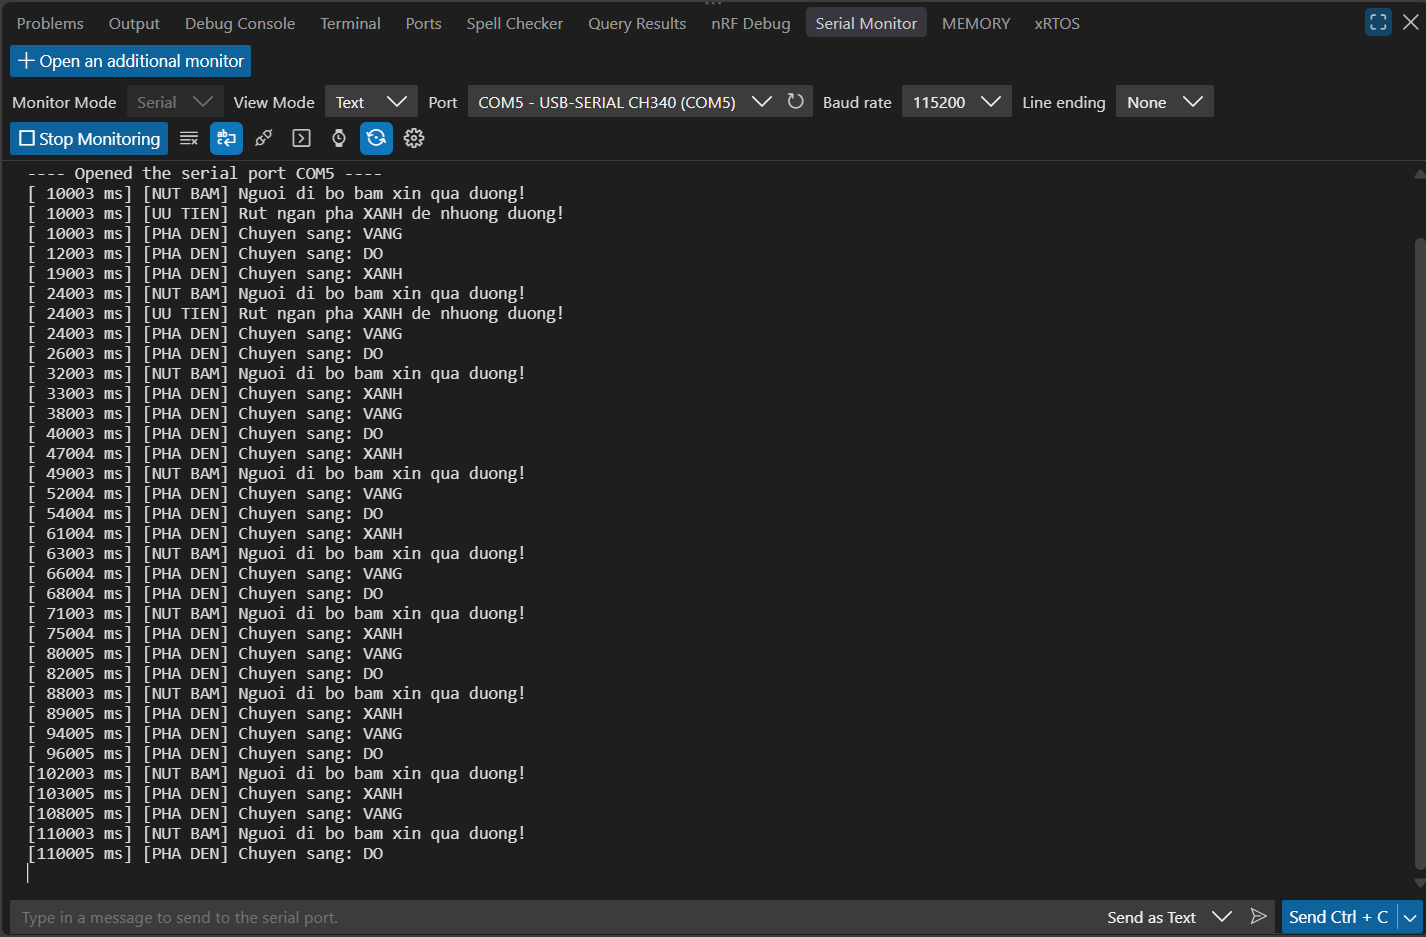
\includegraphics[width=0.92\linewidth]{image/image6.png}
    \caption{Minh chứng log Serial Monitor trên kit thật (115200 baud) - Bài 5}
\end{figure}

\subsubsection{Trả lời câu hỏi bài tập}
\begin{enumerate}[label=(\alph*)]
    \item \textbf{Vì sao cần \texttt{k\_sem\_reset} trước khi chờ yêu cầu trong pha XANH? Cho ví dụ cụ thể từ log nếu bỏ lệnh này.} \\
    \textbf{Trả lời:}
    \begin{itemize}
        \item \textbf{Vì sao cần \texttt{k\_sem\_reset}:} Đèn giao thông chỉ ưu tiên cho người đi bộ khi yêu cầu được bấm trong lúc đèn xe đang XANH (sau 2 giây an toàn bắt buộc ban đầu). Nếu người đi bộ bấm nút lúc xe đang đèn Đỏ hoặc trong 2 giây đầu của đèn Xanh, yêu cầu đó là không hợp lệ. Hàm \texttt{k\_sem\_reset(\&ped\_sem)} đưa semaphore về 0 để xóa sạch các lần bấm cũ không hợp lệ trước đó, bảo đảm luồng chỉ phản ứng với yêu cầu mới phát sinh trong 3 giây tiếp theo.
        \item \textbf{Ví dụ cụ thể từ log nếu bỏ lệnh này:}
        \begin{itemize}
            \item Tại mốc $32000\text{ ms}$ ($32\text{s}$), nút bấm được kích hoạt khi hệ thống đang ở \textbf{PHA ĐỎ} (từ $26\text{s}$ đến $33\text{s}$).
            \item Đến $33000\text{ ms}$ đèn chuyển sang \textbf{PHA XANH} và chạy 2 giây an toàn bắt buộc (đến $35\text{s}$).
            \item \textbf{Nếu BỎ \texttt{k\_sem\_reset}:} Đúng tại $35000\text{ ms}$, lệnh \texttt{k\_sem\_take} sẽ lấy ngay tín hiệu cũ từ lúc $32\text{s}$ và rút ngắn pha xanh ngay lập tức $\rightarrow$ Đèn xanh chỉ sáng được đúng 2 giây đã chuyển sang Vàng, xe cộ vừa xuất phát đã bị ép dừng đột ngột gây tai nạn nguy hiểm.
            \item \textbf{Có \texttt{k\_sem\_reset}:} Tín hiệu lúc $32\text{s}$ bị xóa, đèn XANH sáng trọn vẹn 5 giây (đến $38\text{s}$) trước khi chuyển sang Vàng.
        \end{itemize}
    \end{itemize}
    
    \item \textbf{Vì sao dùng một thread logger duy nhất thay vì để mọi thread tự \texttt{printf}? Vì sao logger nên có ưu tiên thấp nhất?} \\
    \textbf{Trả lời:}
    \begin{itemize}
        \item \textbf{Vì sao dùng một thread logger duy nhất:}
        \begin{itemize}
            \item \textbf{Tránh xung đột ngoại vi UART:} Cổng Serial UART là tài nguyên chia sẻ phần cứng. Nếu nhiều thread cùng gọi \texttt{printf()}, các ký tự sẽ bị xen kẽ làm hỏng dòng log in ra.
            \item \textbf{Bảo đảm tính thời gian thực (Real-time determinism):} Hàm \texttt{printf()} qua UART rất chậm. Sử dụng Message Queue với \texttt{k\_msgq\_put(..., K\_NO\_WAIT)} giúp các thread điều khiển và ISR chỉ mất vài micro-giây để đẩy sự kiện vào hàng đợi rồi quay lại làm việc ngay, không bị trễ thời gian điều khiển.
        \end{itemize}
        \item \textbf{Vì sao logger nên có ưu tiên thấp nhất (Priority 10):} Việc in thông tin ra màn hình chỉ là tác vụ phụ (giám sát). Các tác vụ điều khiển đèn giao thông an toàn (\texttt{Priority 5}) và báo nhịp tim hệ thống (\texttt{Priority 7}) phải luôn được ưu tiên CPU cao hơn. Đặt logger ở mức thấp nhất bảo đảm nó chỉ chạy khi các tác vụ quan trọng đã xử lý xong hoặc đang ngủ.
    \end{itemize}
    
    \item \textbf{Vẽ (hoặc mô tả) dòng thời gian 0–40 s: các pha đèn, các thời điểm có yêu cầu, và những lần pha XANH bị rút ngắn.} \\
    \textbf{Trả lời:}
    
    Bảng dưới đây mô tả chi tiết dòng thời gian diễn biến hệ thống trong khoảng $0 - 40\text{ s}$:
    
    \vspace{0.2cm}
    \small
    \begin{tabularx}{\linewidth}{|>{\centering\arraybackslash}p{2cm}|>{\centering\arraybackslash}p{1.9cm}|>{\centering\arraybackslash}p{2.1cm}|X|}
    \hline
    \textbf{Thời gian} & \textbf{Pha đèn} & \textbf{Sự kiện nút} & \textbf{Diễn biến và Trạng thái} \\
    \hline
    $0\text{s} - 7\text{s}$ & ĐỎ (7s) & Chưa có & Y0 bật sáng, Y1 tắt. Chạy trọn vẹn 7s. \\
    \hline
    $7\text{s} - 10\text{s}$ & XANH (Rút ngắn) & Có tại $t=10\text{s}$ & $7\text{s}-9\text{s}$: Xanh an toàn (2s). Tại $t=10\text{s}$ có yêu cầu $\rightarrow$ \textbf{Rút ngắn pha Xanh ngay lập tức}! \\
    \hline
    $10\text{s} - 12\text{s}$ & VÀNG (2s) & Không & Cả Y0 và Y1 cùng bật sáng trong 2s. \\
    \hline
    $12\text{s} - 19\text{s}$ & ĐỎ (7s) & Không & Y0 bật sáng trong 7s. \\
    \hline
    $19\text{s} - 24\text{s}$ & XANH (5s) & Không có trong cửa sổ & Không có ai bấm trong cửa sổ $21\text{s}-24\text{s}$. Pha xanh chạy trọn vẹn 5s. \\
    \hline
    $24\text{s} - 26\text{s}$ & VÀNG (2s) & Có tại $t=24\text{s}$ & Yêu cầu lần 2 rơi trúng lúc đèn Vàng $\rightarrow$ Bị bỏ qua, không rút ngắn. Cả Y0 và Y1 sáng trong 2s. \\
    \hline
    $26\text{s} - 33\text{s}$ & ĐỎ (7s) & Có tại $t=32\text{s}$ & Y0 sáng. Yêu cầu lần 3 rơi vào đèn Đỏ $\rightarrow$ Sẽ bị \texttt{k\_sem\_reset} xóa bỏ ở giây 35. \\
    \hline
    $33\text{s} - 38\text{s}$ & XANH (5s) & Không có yêu cầu mới & $33\text{s}-35\text{s}$: Xanh an toàn. Tại 35s reset xóa yêu cầu ở giây 32. Không ai bấm mới $\rightarrow$ Chạy trọn vẹn 5s. \\
    \hline
    $38\text{s} - 40\text{s}$ & VÀNG (2s) & Không & Cả Y0 và Y1 cùng bật sáng trong 2s. \\
    \hline
    \end{tabularx}

    \vspace{0.2cm}
    \noindent\textbf{Kết luận:} Trong khoảng $0 - 40\text{ giây}$, chỉ có \textbf{duy nhất 1 lần pha XANH bị rút ngắn} tại mốc \textbf{10000 ms (giây thứ 10)}.
\end{enumerate}
